%
% ####################################################################################################################################################################################
% ####################################################################################################################################################################################
% ####################################################################################################################################################################################
% ####################################################################################################################################################################################
%

\documentclass[]{myHOWTO-V001}


%
% ####################################################################################################################################################################################
% ####################################################################################################################################################################################
%

\usepackage{myTCB-V001}

%
% ####################################################################################################################################################################################
% ####################################################################################################################################################################################
%

\title{The \textbf{myTCB-V1} Package\\{\small Figures}}
\version{1.00}
\author{Norbert EHART (norbert@ehart.net)}
\date{\today}

%
% ####################################################################################################################################################################################
% ####################################################################################################################################################################################
% ####################################################################################################################################################################################
% ####################################################################################################################################################################################
%

\begin{document}
	
%
% ####################################################################################################################################################################################
% ####################################################################################################################################################################################
%

\selectlanguage{english}

%
% ####################################################################################################################################################################################
% ####################################################################################################################################################################################
%

\maketitle

%
% ####################################################################################################################################################################################
% ####################################################################################################################################################################################
%

\tableofcontents

%
% ####################################################################################################################################################################################
% ####################################################################################################################################################################################
%

\section{Introduction}

Latex is mainly used in scientific fields such as electrical engineering, mechanical engineering and computer science. Especially in these fields it is sometimes necessary that certain text sections are explained with a graphic.

\begin{myBOX}{}

\setlength{\parskip}{3mm}

\lipsum[4]

\qquad
\begin{myFIG}{}
	
\includegraphics[scale=0.15]{LaTeX.jpg}
\end{myFIG}

\lipsum[1]

\end{myBOX}

The \emph{myTCB-V1} package provides an environment for this.

\newpage

The \emph{myTCB-V1} package loads automatically the packages shown in \styref{loadingpackages}.

\begin{mySTYdoclst}{Packages}{label={sty:loadingpackages}}
\RequirePackage{lipsum}

\RequirePackage{graphicx}
\RequirePackage{wrapfig}

\RequirePackage{xcolor}

\RequirePackage{verbatim}
\RequirePackage{fancyvrb}
\RequirePackage{listings}

\RequirePackage{float}

\RequirePackage{refstyle}

\RequirePackage{tcolorbox}
	\tcbuselibrary{skins,breakable,listings,xparse}
\end{mySTYdoclst}

To load the package, write \Verb|\usepackage{myTCB-V1}| in the preamble of your document. To use this package, it is highly recommended to have the complete \LaTeX{} distribution installed. This will avoid problems with dependencies.

\begin{myTEXEXdoclst}{Loading myTCB-V1}{label={texex:loadingmyTCBv1}}
\usepackage{myTCB-V1}
\end{myTEXEXdoclst}
	
%
% ####################################################################################################################################################################################
% ####################################################################################################################################################################################
%

\section{The Figure Environment without a List Index}

The \emph{myTCB-V1} package has a predefined environment, which is called \Verb|myFIG|. In this environment there is no list index available and no captions are created.

\begin{myTEXEXdoclst}{}{listing and text}
\setlength{\parskip}{3mm}

\lipsum[4]

\qquad
\begin{myFIG}{}
	
\includegraphics[scale=0.15]{LaTeX.jpg}
\end{myFIG}

\lipsum[2]
\end{myTEXEXdoclst}

\newpage

A title can be submitted as an optional argument, which appears in the lower center part of the box.

\begin{myTEXEXdoclst}{}{listing and text}
\setlength{\parskip}{3mm}

\lipsum[4]

\qquad
\begin{myFIG}{title={This is a picture}}
	
\includegraphics[scale=0.15]{LaTeX.jpg}
\end{myFIG}

\lipsum[2]
\end{myTEXEXdoclst}

%
% ####################################################################################################################################################################################
% ####################################################################################################################################################################################
%

\section{The Figure Environment with a List Index}

The \emph{myTCB-V1} package has a predefined environment, which is called \Verb|myFIGlst|. In this environment is a list index available. A title (\verb|TITLE1|) must be passed as a mandatory argument. This title does not appear on the box, instead it is found in the list index. The box itself is titled with \emph{Figure} and a sequential number.

\begin{myTEXEXdoclst}{}{listing and text}
\setlength{\parskip}{3mm}

\lipsum[4]

\qquad
\begin{myFIGlst}{TITLE1}{}
	
\includegraphics[scale=0.15]{LaTeX.jpg}
\end{myFIGlst}

\lipsum[2]
\end{myTEXEXdoclst}

\begin{minipage}{0.46\linewidth}
\centering
\begin{myFIGlst}{myBOX LoF}{label={fig:myfiglofdef}}
	\includegraphics[page=1,scale=0.18]{examples/myFIGV000.pdf}
\end{myFIGlst}
\end{minipage}
\begin{minipage}{0.46\linewidth}
You can create the list index with the command \Verb|\listofmyFIG|.
\\

\begin{myTEXEXdoclst}{}{label={texex:mystylistentry}, listing only}
\listofmyFIG
\end{myTEXEXdoclst}

This will create a list index which looks like the picture in \figref{myfiglofdef}. 
\end{minipage}

If you want to change the horizontal spacing of the list entries, you can do this quite simple with the following code in the preamble, which is illustrated in \texexref{horispacefig}.

\begin{myTEXEXdoclst}{}{label={texex:horispacefig}, listing only}
\makeatletter
	\renewcommand{\l@myFIG}{\@dottedtocline{1}{0mm}{0mm}}
\makeatother
\end{myTEXEXdoclst}

If you want to change the vertical spacing of the list entries, you can do this quite simple with the following code in the preamble, which is illustrated in \texexref{vertspacfig}.

\begin{myTEXEXdoclst}{}{label={texex:vertspacfig}, listing only}
\makeatletter
	\addtocontents{myFIG}{\protect\vspace{12mm}}
\makeatother
\end{myTEXEXdoclst}

If you want to get rid of the page numbers in the list index, you can do this quite simple with the following code in the preamble, which is illustrated in \texexref{getridheadfootmyfig}.

\begin{myTEXEXdoclst}{}{label={texex:getridheadfootmyfig}, listing only}
% copy cmd \listofmyFIG into cmd \oldlistofmyFIG
\let\oldlistofmyFIG\listofmyFIG

% renew cmd \listofmyFIG
\renewcommand\listofmyFIG
{
	\pagestyle{empty} % .... % disable headers/footers
	\oldlistofmyFIG % ...... % call \oldlistofmyFIG
	\clearpage % ........... % create a new page
	\pagestyle{plain} % .... % enable headers/footers; use fancy if you use fancyhdr
}
\end{myTEXEXdoclst}

A label can be specified as an optional argument. The box can then be referenced in the text with \Verb|\figref{}|.

\begin{myTEXEXdoclst}{}{listing and text}
\centering
\begin{myFIGlst}{TITLE2}{label={fig:FIG001}}
	
\includegraphics[scale=0.15]{LaTeX.jpg}
\end{myFIGlst}
\end{myTEXEXdoclst}

\begin{myTEXEXdoclst}{}{listing and text}
This example is shown in \figref{FIG001}
\end{myTEXEXdoclst}

It is notable that the label has to contain the \Verb|fig:| prefix in order to reference the label appropriately.

%
% ####################################################################################################################################################################################
% ####################################################################################################################################################################################
%

\section{Images}

Images are essential elements in most of the scientific documents. \LaTeX{} provides several options to handle images and make them look exactly what you need. \cite{Overleaf2023}

\LaTeX{} can not manage images by itself, so we need to use the \emph{graphicx} package. \cite{Overleaf2023}

To use it, we include the following line in the preamble. 

\begin{myTEXEXdoclst}{}{}
\usepackage{graphicx}
\end{myTEXEXdoclst}

The \Verb|\includegraphics{file}| command is the one that actually included the image in the document. Here \emph{file} is the name of the file containing the image without the extension, then file.PNG becomes universe. The file name of the image should not contain white spaces nor multiple dots. The file extension is allowed to be included, but it's a good idea to omit it. If the file extension is omitted it will prompt LaTeX to search for all the supported formats. \cite{Overleaf2023}

The path inside the command \Verb|\includegraphics{file}| has to be relative to the current working directory or absolute.

The command \Verb|
\includegraphics[scale=0.07]{LaTeX}| will include the image \Verb|LaTeX| in the document, the extra parameter \Verb|scale=0.07| will do exactly that, scale the image 7\% of its real size.

\begin{myTEXEXdoclst}{}{listing and text}
\setlength{\parskip}{3mm}

This is an example.

\centering
\begin{myFIGlst}{TITLE2}{}
	
\includegraphics[scale=0.07]{LaTeX.jpg}
\end{myFIGlst}

\justifying
We see here how it actually works.
\end{myTEXEXdoclst}

With \Verb|\centering| we center everything after the command. With \Verb|\justifying| we switch back to the default alignment. Instead of \Verb|\centering|, you can use other methods for horizontal text alignment. There are several methods in \LaTeX{} to do this.

\begin{itemize}
	\item create a small space (\Verb|\,|)
	\item create a medium space (\Verb|\:|)
	\item create a large space (\Verb|\;|)
	\item create a really large space (\Verb|\quad|)
	\item create a huge space (\Verb|\qquad|)
	\item create a negative space (\Verb|\!|)
	\item create a space that have a specific length (\Verb|\hspace{3mm}|)
	\item create as much horizontal space as possible (\Verb|\hfill|)
\end{itemize}

It is notable that after a whitespace creation, we do not need to switch back to the default with \Verb|\justifying|.

You can also scale the image to a some specific \Verb|width| and \Verb|height|. \cite{Overleaf2023}

\begin{myTEXEXdoclst}{}{listing and text}
\centering
\begin{myFIGlst}{TITLE2}{}
	
\includegraphics[width=80mm]{LaTeX.jpg}
\end{myFIGlst}
\end{myTEXEXdoclst}

If only the \Verb|width| parameter is passed, the \Verb|height| will be scaled to keep the aspect ratio. \cite{Overleaf2023}

The same rule applies if only the \Verb|height| parameter is passed.

\begin{myTEXEXdoclst}{}{listing and text}
\centering
\begin{myFIGlst}{TITLE2}{}
	
\includegraphics[height=40mm]{LaTeX.jpg}
\end{myFIGlst}
\end{myTEXEXdoclst}

The length units can also be relative to some elements in document. If you want, for instance, make a picture the same width as the text. \cite{Overleaf2023}

\begin{myTEXEXdoclst}{}{listing and text}
\centering
\begin{myFIGlst}{TITLE2}{}
	
\includegraphics[width=0.9\textwidth]{LaTeX.jpg}
\end{myFIGlst}
\end{myTEXEXdoclst}

Another common option is the angle option to rotate the image.

\begin{myTEXEXdoclst}{}{listing and text}
\centering
\begin{myFIGlst}{TITLE2}{}
	
\includegraphics[width=80mm, angle=20]{LaTeX.jpg}
\end{myFIGlst}
\end{myTEXEXdoclst}

\newpage

It's also possible to wrap the text around a figure. When the document contains small pictures this makes it look better. \cite{Overleaf2023}

\begin{myTEXEXdoclst}{}{listing and text}
\vspace{5mm}
\section*{Test Page}
\begin{wrapfigure}{l}{0.45\textwidth}
	\centering
	\begin{myFIGlst}{TITLE3}{}
		
\includegraphics[scale=0.1]{LaTeX.jpg}
	\end{myFIGlst}
\end{wrapfigure}
\lipsum[4] \lipsum[4]
\end{myTEXEXdoclst}

To use wrapfig, include the following line in the document preamble.

\begin{myTEXEXdoclst}{}{}
\usepackage{wrapfig}
\end{myTEXEXdoclst}

\newpage

To crop images, you can use the \emph{trim} option of the \emph{graphicx} package. The option \emph{trim} expects 4 values, which are the lengths that should be trimmed from the left, bottom, right and top side. After setting these values you must activate the cropping with \emph{clip}. If you combine trim with height or something similar the image will be cropped and then resized.

\begin{myTEXEXdoclst}{}{listing and text}
\centering
\begin{myFIGlst}{TITLE2}{}
	
\includegraphics[scale=0.15,trim=80mm 80mm 80mm 60mm,clip]{LaTeX.jpg}
\end{myFIGlst}
\end{myTEXEXdoclst}

You can even insert a PDF file (on a specific page) with the \emph{graphicx} package.

\begin{myTEXEXdoclst}{}{listing and text}
\centering
\begin{myFIGlst}{TITLE2}{}
	\includegraphics[page=2, scale=0.22, trim=20mm 20mm 20mm 20mm, clip]{myFIGV000.pdf}
\end{myFIGlst}
\end{myTEXEXdoclst}

\newpage

You can also put 2 pictures side by side.

\begin{myTEXEXdoclst}{}{listing and text}
\centering
\begin{myFIGlst}{TITLE2}{}
	
\includegraphics[scale=0.15,trim=80mm 80mm 80mm 60mm,clip]{LaTeX.jpg}
	
\includegraphics[scale=0.15,trim=80mm 80mm 80mm 60mm,clip]{LaTeX.jpg}
\end{myFIGlst}
\end{myTEXEXdoclst}

%
% ####################################################################################################################################################################################
% ####################################################################################################################################################################################
%

\clearpage
\pagestyle{empty}
\printbibliography[heading=bibnumbered]
\clearpage
\pagestyle{plain}

%
% ####################################################################################################################################################################################
% ####################################################################################################################################################################################
%
	
\end{document}

%
% ####################################################################################################################################################################################
% ####################################################################################################################################################################################
% ####################################################################################################################################################################################
% ####################################################################################################################################################################################
%